\documentclass[conference]{IEEEtran}
\IEEEoverridecommandlockouts
% The preceding line is only needed to identify funding in the first footnote. If that is unneeded, please comment it out.
\usepackage{cite}
\usepackage{amsmath,amssymb,amsfonts}
\usepackage{algorithmic}
\usepackage{graphicx}
\usepackage{textcomp}
\usepackage{xcolor}
\def\BibTeX{{\rm B\kern-.05em{\sc i\kern-.025em b}\kern-.08em
    T\kern-.1667em\lower.7ex\hbox{E}\kern-.125emX}}
\begin{document}

\title{Breast Cancer  Prediction Using Machine  Learning \\
{\footnotesize \textsuperscript{}}
\thanks{https://github.com/SriLakshmi1128/MLProject


https://github.com/MallulaGowtham/MLproject}
}

\author{\IEEEauthorblockN{1\textsuperscript{st} Chereddy Sri Lakshmi}

\and
\IEEEauthorblockN{2\textsuperscript{nd} Mallula Gowtham}

}

\maketitle

\begin{abstract}
Breast cancer is one of the most dreaded and commonly occurring malignancies currently among women, affecting around 10\% of women worldwide at different stages of their lives [1]. The biggest problem arises when the disease cannot be accurately diagnosed at the very early stages, despite the fact that the treatment for this illness is now accessible in practice in many countries. In this area, machine learning has proven to be essential in predicting illnesses like cancer. Data classification techniques such as data mining have shown to be reliable and efficient thus far. These techniques have been utilized, particularly in the realm of medicine, to detect diseases.  In this paper, we have successfully used six classification techniques in the form of  K-Neighbors, Logistic Regression, Naïve Bayes and Support Vector Machine (SVM), Random Forest classifier on the Wisconsin Breast Cancer (original) datasets, both before and after applying Principal Component 
analysis. The main objective is to assess the correctness in classifying data with respect to the efficiency and effectiveness of each algorithm in terms of accuracy, precision, recall, specificity and F1 Score. 
\end{abstract}

\begin{IEEEkeywords}
Decision tree, Machine learning, Support vector machine, Recall, 10-Fold cross-validation
\end{IEEEkeywords}

\section{Introduction}
Breast cancer (BC) is the most common cancer in women, affecting about 10 percent of all women at some stages of their life. In modern times, the rate keeps increasing and data show that the survival rate is 88 percent after five years from diagnosis and 80 percent after 10 years from diagnosis. Early prediction of breast cancer so far have made heaps of improvement, death rate of breast cancer by 39 percent, starting from 1989.. Due to varying nature of breast cancers symptoms, patients are often subjected to a barrage of tests, including but not limited to mammography, ultrasound and biopsy, to check their likelihoods of being diagnosed with breast cancer. Biopsy, is the most indicative among these procedures, which involves extraction of sample cells or tissues for examination. The sample of cells is obtained from a breast fine needle aspiration (FNA) procedure and then sent to a pathology laboratory to be examined under a microscope [12]. Numerical features, such as radius, texture, perimeter and area, can be measured from microscopic images. Data, later on, obtained from FNA are analyzed in combination with various imaging data to predict probability of the patient having malignant breast cancer tumor. An automated system here would be hugely beneficial in this scenario. It will likely expedite the process and enhance the accuracy of the doctor’s predictions. In addition, if supported by abundance dataset and the automated system consistently performs well, it will potentially eliminate  he needs for patients to go through various other tests, such as mammography, ultrasound, and MRI, which subject patients to significant amount of pain and radiation. In all, early
prediction remains is one of the vital aspects in the follow-up process. Data mining methods or classification can help to reduce the number of false positive and false negative decisions. Consequently, new ways like data discovery in databases (KDD) has become a preferred tool for medical researcher. In this paper, using six classification models; Decision Tree, K-Neighbors, Linear Discriminant Analysis (LDA), Logistic Regression, Naïve Bayes and Support Vector Machine (SVM) have been run on the Wisconsin Breast Cancer (original) datasets, both before and after applying Principal Component Analysis. The results obtained are then measured using various performance metrics to compare among the algorithms in order to find out the best-suited model for cancer prediction.

This cancer may be a quite common sort of cancer among girls and therefore the
second highest reason behind cancer death. Within the United State, regarding one in eight girls over their time period includes a risk of developing breast cancer. With the uncontrolled division of one cell inside the breast leads to beginning to the breast cancer which results in a visible mass, called a tumour. The tumour can be either benign or malignant. The correct designation in determinant whether or not the tumour is benign or malignant may result in saving lives. Therefore, the necessity for precise classification within the clinic may be an explanation for nice concern for specialists and doctors. This importance of Artificial intelligence has been actuated for the last twenty five years, once scientists began to understand the quality of taking bound selections to treat specific diseases. The employment of machine learning and data processing as tools in diagnosing becomes terribly effective and one amongst the crucial diseases in medicines wherever the classification task plays a really essential role is that the diagnosis of breast cancer. 
Therefore, machine learning techniques will facilitate doctors to create an correct identification for breast cancer and make the proper classification of being benign or malignant tumor. There is little question that analysis of information taken from the patient and selections of doctors and specialists are the foremost necessary factors within the identification, however knowledgeable systems and artificial intelligence techniques like machine learning for classification tasks, conjointly facilitate doctors and specialists in a great deal.

\section{Motivation}
Breast cancer is one of the most common cancer in women and the second leading cause of women’s cancer death[1]. Despite the lack of effective treatment, the low accuracy of diagnosis is also a major cause of the high incidence and mortality of breast cancer. Mammography is a traditional method used for diagnosing breast cancer. According to UCHealth’s report, only 78\% of breast cancer can be accurately diagnosed by mammography [2]. So there is a need of building an expert system for early diagnosis of breast cancer.

\section{Objectives}
\begin{itemize}
    \item To clean and prepare the data effectively to train the machine learning model, cleaning data by deleting the rows missing values or null values.
    \item To implement and evaluate the classification models available in machine learning for the considered breast cancer dataset. 
\end{itemize}
The Machine learning algorithms that we trained for the breast cancer dataset are:
\begin{itemize}
  \item Logisitc regression
  \item Support Vector Machine
  \item K - Nearest Neighbors
  \item Naive Bayes
  \item Random forest
\end{itemize}

\section{Related work}

Earlier, research regarding the classification and prediction of breast cancer has been carried out using several data mining techniques. Classification and agglomeration are 2 widely used ways in information mining [1].
Classification also known as supervised learning in machine learning, aims to classify unknown things supported learning existing patterns and classes from the information set and after predicting future things. The training set, that is employed to build the classifying structure, and therefore the take-a-look-at set, that tends to assess the classifier, are ordinarily mentioned in
classification tasks [2].

Furthermore, essential progress has been carried out when it comes to breast cancer survivability prediction using labeled, unlabeled, and pseudo-labeled patient data. Prognostic studies of breast cancer survivability have been aided by machine learning algorithms, which can predict the survival of a particular patient based on historical patient data. Neural networks and related techniques have a vast contribution when it comes to predicting breast cancer. Over the past few decades, Artificial Neural Networks have been employed increasingly by more and more researchers, and become an active research area [7-12]. 

ANNs have afforded numerous successes with great progress in Breast Cancer classification and diagnosis in the very early stages [2,7-12]. A typical ANN model is made up of a hierarchy of layers: input, hidden, and output layers. Extensive research had been done with the backpropagation artificial neural network (BP-ANN) method and its variations in breast cancer diagnosis [13]–[14]. The technique, however, has some limitations such as no guarantee to global optima, a lot of tuning parameters, and long training time. Single Hidden Layer Neural Networks (SFLN) was proposed by Huang and Babri [15] to tackle the mentioned problems with tree steps learning process called extreme learning machine (ELM). Standard [16] and best-parameterized [17] ELM models were proposed for breast cancer early prediction. Results showed that it generally gave better accuracy, specificity, and sensitivity compared to BP ANN. 

However, most existing works focus on prediction performance with limited attention with medical professionals as end users and applicability aspects in real medical settings With due respect to all related work referred to above, this paper compares the performance of the algorithms; Decision Tree, K-Neighbors, Logistic Regression, Naïve Bayes, and Support Vector Machine (SVM) using Wisconsin Breast Cancer (original) datasets in both diagnosis and analysis to make decisions. 


\section{Proposed frame work}
With our aim being to predict whether the tumor is Benign (non-cancerous) or Malignant (cancerous), we have outlined a simple model to come with the most accurate predictions. The first objective was to attain a dataset of numerical values of various instances. Upon finalizing our dataset, we split the train-test ration to 70:30 in order to train and test six algorithms: Random forest, K-Neighbors, Logistic Regression, Naïve Bayes and Support Vector machine (SVM). Feature selection in the form of Principal Component Analysis is used to reduce dimensionality of the dataset. The models are trained again by means of training and testing  and finally compared the results with that of the previous results. The workflow below outlines a basic review of the entire thesis:-

\begin{figure}[htbp]
\centerline{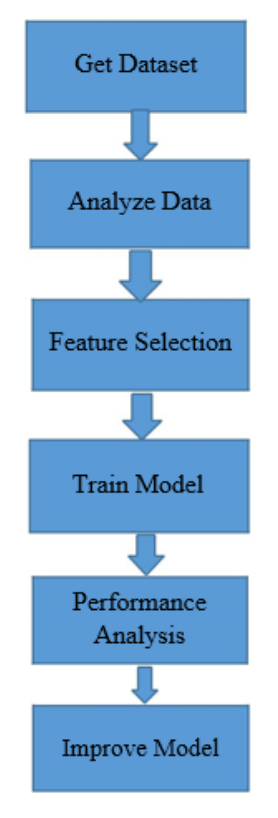
\includegraphics[width=25mm]{proposed.png}}
\caption{Process Flow Diagram}
\label{fig}
\end{figure}

\subsection{Dataset Collection}\label{AA}
The dataset used for this paper is publicly available and was created by Dr. William H. Wolberg, physician at the University Of Wisconsin Hospital at Madison, Wisconsin, United States of America. 
The dataset contains 357 cases of benign breast cancer and 212 cases of malignant breast cancer. The dataset contains 32 columns, with the first column being the ID number, the second column being the diagnosis result (benign or malignant), and followed by the mean, standard deviation and the mean of the
worst measurements of ten features. There were no missing values in the dataset [18].
The columns present in the dataset are:
\begin{figure}[htbp]
\centerline{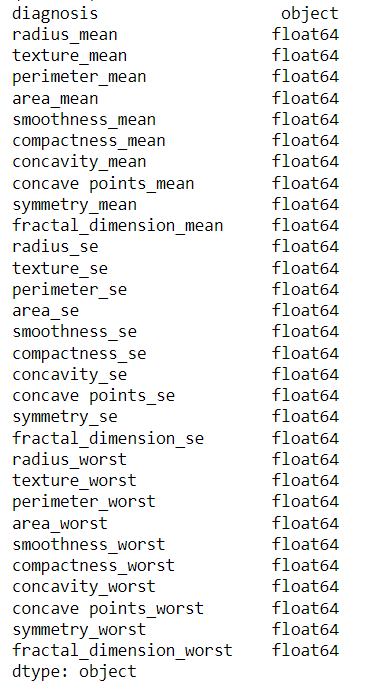
\includegraphics[width=70mm]{dataset.png}}
\caption{Features present in the breast cancer dataset}
\label{fig}
\end{figure} 

\subsection{Feature selction}
Variable selection or attribute selection is known as feature selection. Automatic selection of attributes in the data that are most relevant to the predictive modeling problem. Dimensionality reduction is completely different from feature selection. Each strategies request to scale back the quantity of attributes within the dataset, however a dimensionality reduction methodology do thus by making new combination of attributes, wherever as feature selection strategies embrace and exclude attributes present within the data while not ever-changing them. An accurate predictive model is created by feature selection methods. Helping in choosing features will provide best or better accuracy whilst requiring less data. Identifying and removing unneeded can be done by using the feature selection method.
\begin{figure}[htbp]
\centerline{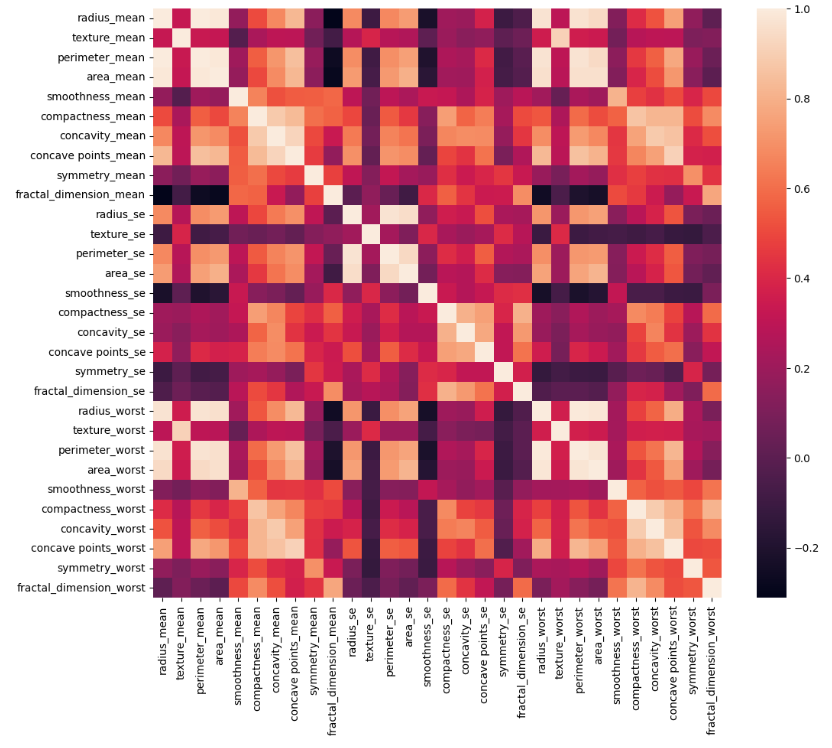
\includegraphics[width=100mm]{correlation.png}}
\caption{Co-efficient correlation matrix}
\label{fig}
\end{figure} 

\subsection{Splitting data for training and validation}
Here in this section we used the sklearn module in python to split our numerical tabular dataset into 2 with 70 percent as training data and remaining as validation data.
\begin{figure}[htbp]
\centerline{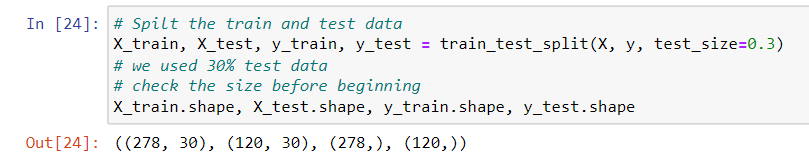
\includegraphics[width=100mm]{split_data.png}}
\caption{Test and train split of data}
\label{fig}
\end{figure}

\subsection{Model building}
Here in this section we used sklearn module from python to implement the machine learning algorithms.

\subsubsection{Logistic Regression}
Logistic regression measures the link between the variable quantity, the output, and therefore the freelance variables, the input. By estimating chances exploitation its underlying supply perform. It uses 1.2 penalty for regularization. Supply regression formula conjointly uses an equation with freelance predictors to predict a worth. The expected worth are often anyplace between negative eternity to positive eternity. The resultant chances are then born-again to binary values zero or one by the supply perform, conjointly referred to as the sigmoid function.
\begin{figure}[htbp]
\centerline{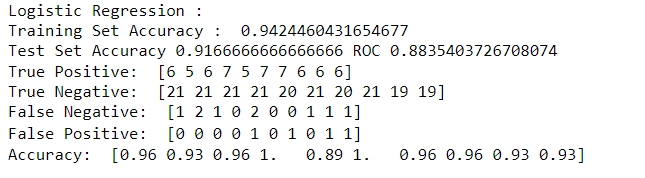
\includegraphics[width=100mm]{logistic.png}}
\caption{Logistic Regression performance}
\label{fig}
\end{figure}

\subsubsection{ Support Vector Machine}
Support Vector Machine (SVM) is a supervised machine learning algorithmic rule which might be used for each classification or regression challenges. However, it’s principally utilized in classification issues. In this algorithmic rule, we plot each data item as a point in n-dimensional space where n is number of features one has with the value of each feature being the value of a particular coordinate [23]. Then, we perform classification by finding the hyper-plane that differentiates the two classes.
\begin{figure}[htbp]
\centerline{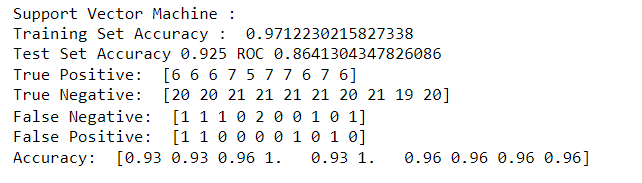
\includegraphics[width=100mm]{svm.png}}
\caption{Support Vector Machine performance}
\label{fig}
\end{figure}

\subsubsection{Naive Bayes classifier}
Naive Bayes classifiers are a group of classification algorithms supported Bayes’ Theorem. It’s not one algorithmic rule however a family of algorithms wherever all of them share a typical principle, each try of options being classified is freelance of every different. Bayes theorem uses the contingent probability that successively uses previous information to calculate the probability that a future event can happen. In Naive Bayes classifier, it’s assumed that the input variables are freelance of every alternative which all options can separately contribute to the chance of target variable.
\begin{figure}[htbp]
\centerline{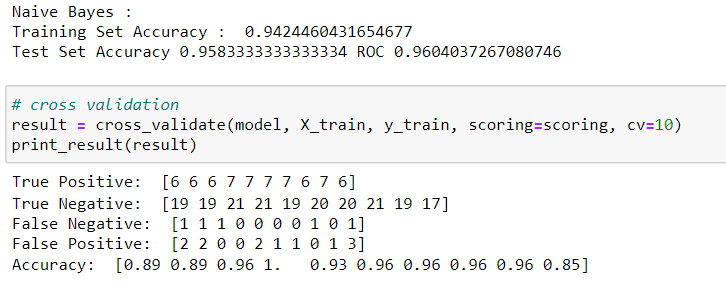
\includegraphics[width=80mm]{naive.png}}
\caption{Naive Bayes classifier performance}
\label{fig}
\end{figure}
 
\subsubsection{Random forest}
Random Forest Regression is a supervised learning algorithm that uses ensemble learning method for regression. Ensemble learning method is a technique that combines predictions from multiple machine learning algorithms to make a more accurate prediction than a single model.
\begin{figure}[htbp]
\centerline{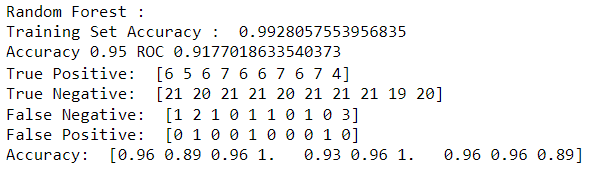
\includegraphics[width=100mm]{random.png}}
\caption{Random forest classifier performance}
\label{fig}
\end{figure}

\subsubsection{KNN Classifer}
The k-nearest neighbors (KNN) algorithm is a data classification method for estimating the likelihood that a data point will become a member of one group or another based on what group the data points nearest to it belong to.
The k-nearest neighbor algorithm is a type of supervised machine learning algorithm used to solve classification and regression problems. However, it's mainly used for classification problems.
\begin{figure}[htbp]
\centerline{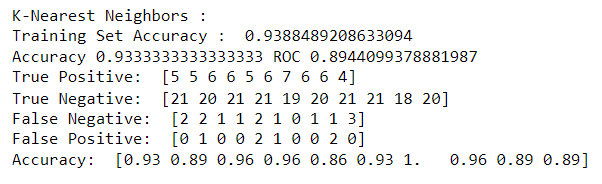
\includegraphics[width=100mm]{knn.png}}
\caption{KNN Classifer performance}
\label{fig}
\end{figure}

\section{Results and Analysis}

The next step after applying implementing machine learning models is to seek out how effective is that the model, i.e. how the models performed on the datasets. This is carried out by running the models on the test dataset which was set earlier. The test dataset comprised of 30\% of the dataset for Breast Cancer prediction.10-fold cross-validation was also done for Breast cancer pre-diction. We evaluated six machine learning algorithms, they are logistic regression, random forest classifier, KNN classifier, Naive Bayes classifier, and  Support vector machine.
\begin{figure}[htbp]
\centerline{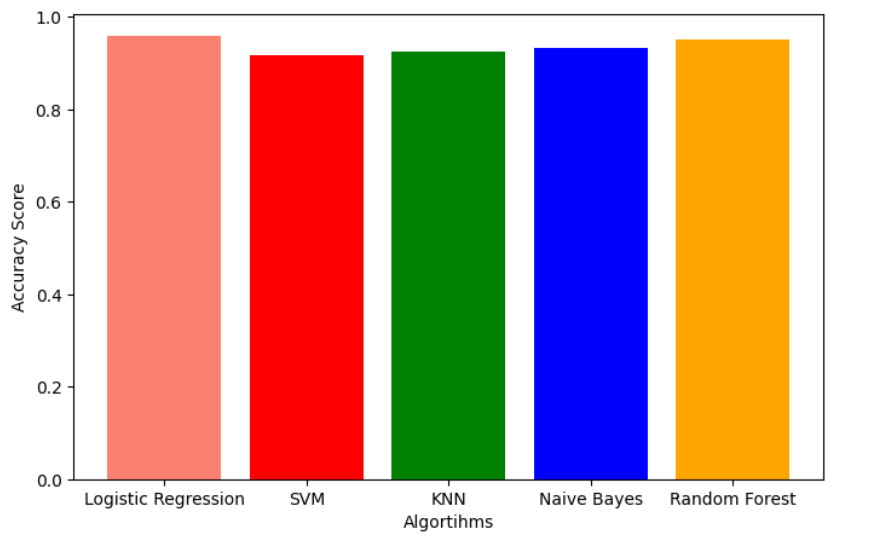
\includegraphics[width=8cm, height=4cm]{accuracy.png}}
\caption{Accuracy graph for the classifiers}
\label{fig}
\end{figure}
\begin{figure}[htbp]
\centerline{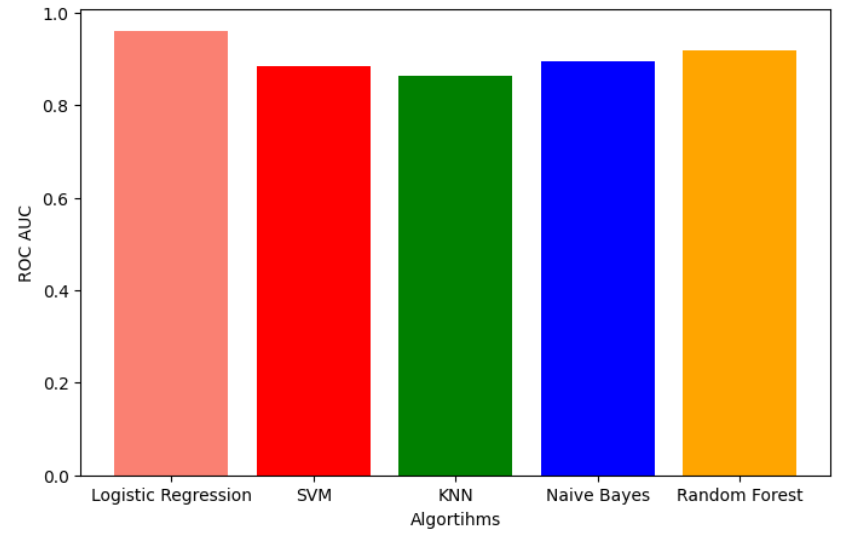
\includegraphics[width=8cm, height=4cm]{roc_auc.png}}
\caption{ROC scores for the different classifiers}
\label{fig}
\end{figure}


\section*{Conclusion}

In terms of accuracy, Naïve Bayes, has scored 0.964. K-Neighbors (0.9349) and Logistic regression (0.923) are not far behind either. SVM scores 0.917 in accuracy. Decision Tree performs the worst among all six resulting 0.834. 
Considering the other performance matrix into account, a lot can be determined regarding the performance of the algorithms. K-Neighbors and Naïve Bayes performs better SVM and Logistic Regression scores a perfect 1.000 when it comes to recall, which is vital in terms of disease prediction, even though there are declines in the values of all other performance metrics of both the mentioned algorithms. keeping the recall score into consideration, we can conclude that Logistic Regression and Support Vector Analysis performs better when it comes to Breast Cancer Prediction for this dataset used.


\begin{thebibliography}{00}
\bibitem{b1}] Breast cancer facts and figures 2003-2004 (2003). American Cancer Society
\bibitem{b2}Stages | Mesothelioma | Cancer Research UK Breast cancer survival statistics September 26, 2017
\bibitem{b3}Pendharkar PC, Rodger JA, Yaverbaum GJ, Herman N, Benner M (1999) Association, statistical, mathematical and neural approaches for mining breast cancer patterns. Expert Systems with Applications 17: 223-232.
\bibitem{b4}deepsense.ai What is reinforcement learning? The complete guide July 05, 2018
\bibitem{b5}Hacker Noon Absolute Fundamentals of Machine Learning – Hacker Noon January 15, 2018
\bibitem{b6} Furundzic, D.; Djordjevic, M.; Bekic, A.J. Neural networks approach to early breast cancer detection. J. Syst. Archit. 1998, 44, 617–633. [CrossRef]
\bibitem{b7}] Floyd, C.E.; Lo, J.Y.; Yun, A.J.; Sullivan, D.C.; Kornguth, P.J. Prediction of breast cancer malignancy using an artificial neural network. Cancer 1994, 74, 2944–2948. [CrossRef]
\bibitem{b8}H. A. Abbass, “An evolutionary artificial neural networks approach fo
\bibitem{b9}J. Khan, J. S. Wei, M. Ringnér, L. H. Saal, M. Ladanyi, F. Westermann, F. Berthold, M. Schwab, C. R. Antonescu, C. Peterson, and P. S. Meltzer, “Classification and diagnostic prediction of cancers using gene expression profiling and artificial neural networks.,” Nat. Med., vol. 7, no.
6, pp. 673–9, Jun. 2001.
\bibitem{b10}  G.-B. Huang, Q.-Y. Zhu, and C.-K. Siew, “Extreme learning machine: Theory and applications,” Neurocomputing, (Dec. 2006.) vol. 70, no. 1–3, pp. 489–501.
\bibitem{b11} C. P. Utomo, A. Kardiana, and R. Yuliwulandari, “Breast Cancer Diagnosis using Artifi-cial Neural Networks with Extreme Learning Techniques,” Int. J. Adv. Res. Artif. Intell, vol. 3, no. 7,pp. 10–14,
\bibitem{12} Fine Needle Aspiration Biopsy of the Breast. American Cancer Society.
\bibitem{13} Friedman, Jerome, Trevor Hastie, and Rob Tibshirani. Regularization paths for generalized linear models via coordinate descent.” Journal of statistical software 33.1 (2010): 1
\bibitem{14}Rohith Gandhi. Nearest Neighbor. Understanding Machine Learning (2018)
\bibitem{15} Machine Learning Mastery Discriminant Analysis for Machine Learning September 22, (2016)

\bibitem{16} G.-B. Huang, Q.-Y. Zhu, and C.-K. Siew, “Extreme learning machine: Theory and applications,” Neurocomputing, (Dec. 2006.) vol. 70, no. 1–3, pp. 489–501.
\bibitem{17} C. P. Utomo, A. Kardiana, and R. Yuliwulandari, “Breast Cancer Diagnosis using Artifi-cial Neural Networks with Extreme Learning Techniques,” Int. J. Adv. Res. Artif. Intell, vol. 3, no. 7, pp. 10–14
\bibitem{18} William H Wolberg, W Nick Street, and Olvi L Mangasarian. (1992). Breast cancer Wisconsin (diagnostic) data set. UCI Machine Learning Repository.
\bibitem{19}H. A. Abbass, “An evolutionary artificial neural networks approach for breast cancer diagnosis.” Artif.Intell. Med., vol. 25, no. 3, pp. 265–81,
\bibitem{20} J. Khan, J. S. Wei, M. Ringnér, L. H. Saal, M. Ladanyi, F. Westermann, F. Berthold, M. Schwab, C. R. Antonescu, C. Peterson, and P. S. Meltzer, “Classification and diagnostic prediction of cancers using gene expression profiling and artificial neural networks.,” Nat. Med., vol. 7, no.
6, pp. 673–9
\end{thebibliography}


\end{document}


